\section{Bibliography Review}
\label{sec:bibliography-review}

A bibliographical research was performed to determine the state of the art in the field of the project,
both in terms of the models and algorithms used as well as the chosen state and action spaces which perform best
with regard to realistic environment simulations.
The search was made using the Web of Science repository, covering the last 5 years, with the following search key:

\begin{verbatim}
    (
        "reinforcement learning" OR "dynamic programming" OR
        "optimal control" OR "control theory" OR "machine learning"
    )
    AND
    (
        "market making" OR "market maker"
    )
\end{verbatim}

Initially, 64 references were selected and deemed relevant to the project, with 23 of them being selected for further analysis and effectively used in our analysis,
and 4 additional references being added to the list after the initial selection.
The references were selected based on their relevance to the project and tagged according to the following groups
(for each non-binary category, combinations of tags were allowed):

\begin{itemize}
    \item Type of data (simulated, real-time connections, and others);
    \item Chosen state space (vectors of bid-ask spreads, order imbalance, N-depth order books, and others);
    \item Chosen action space (limit orders, market orders, and others);
    \item Chosen Reward space (spread, volume, profit, and others);
    \item Algorithms used (Q-Learning, Deep Q-Learning, Actor-Critic, or others);
    \item Whether a multi-agent approach was used (dueling or market agents);
    \item If a model-free environment was used (model-based or model-free);
    \item Metrics used for comparison (Sharpe Ratio, PnL, and others).
    \item Finally, results were tagged by their benchmarks, that is, the strategies used for comparison.
\end{itemize}

\subsection{State, Action, and Reward Spaces}

State-of-the-art references defined state spaces primarily based on market-level observations,
specifically top-of-book quotes and n-depth book levels which align well with the real-time data available to market-making agents \cite{he2023integrating, bakshaev2020marketmaking}.
Additionally, agent inventory was also a common feature, reflecting the importance of managing risk and liquidity in market-making strategies \cite{patel2018optimizing, ganesh2019reinforcement}.
Action spaces included possible multiple bid-ask spreads or just one pair of quotes. Some references also used discrete book levels as actions.

\begin{figure}[H]
    \centering
    % graph: images/state_space.png
    \makebox[\textwidth][c]{%
        \begin{subfigure}{.5\textwidth}
            \centering
            \includegraphics[width=\textwidth]{images/reward_space}
            \caption{State Space 3}
            \label{fig:figure3}
        \end{subfigure}
        \hspace{0.02\textwidth} % Adjust spacing between figures
        \begin{subfigure}{0.5\textwidth}
            \centering
            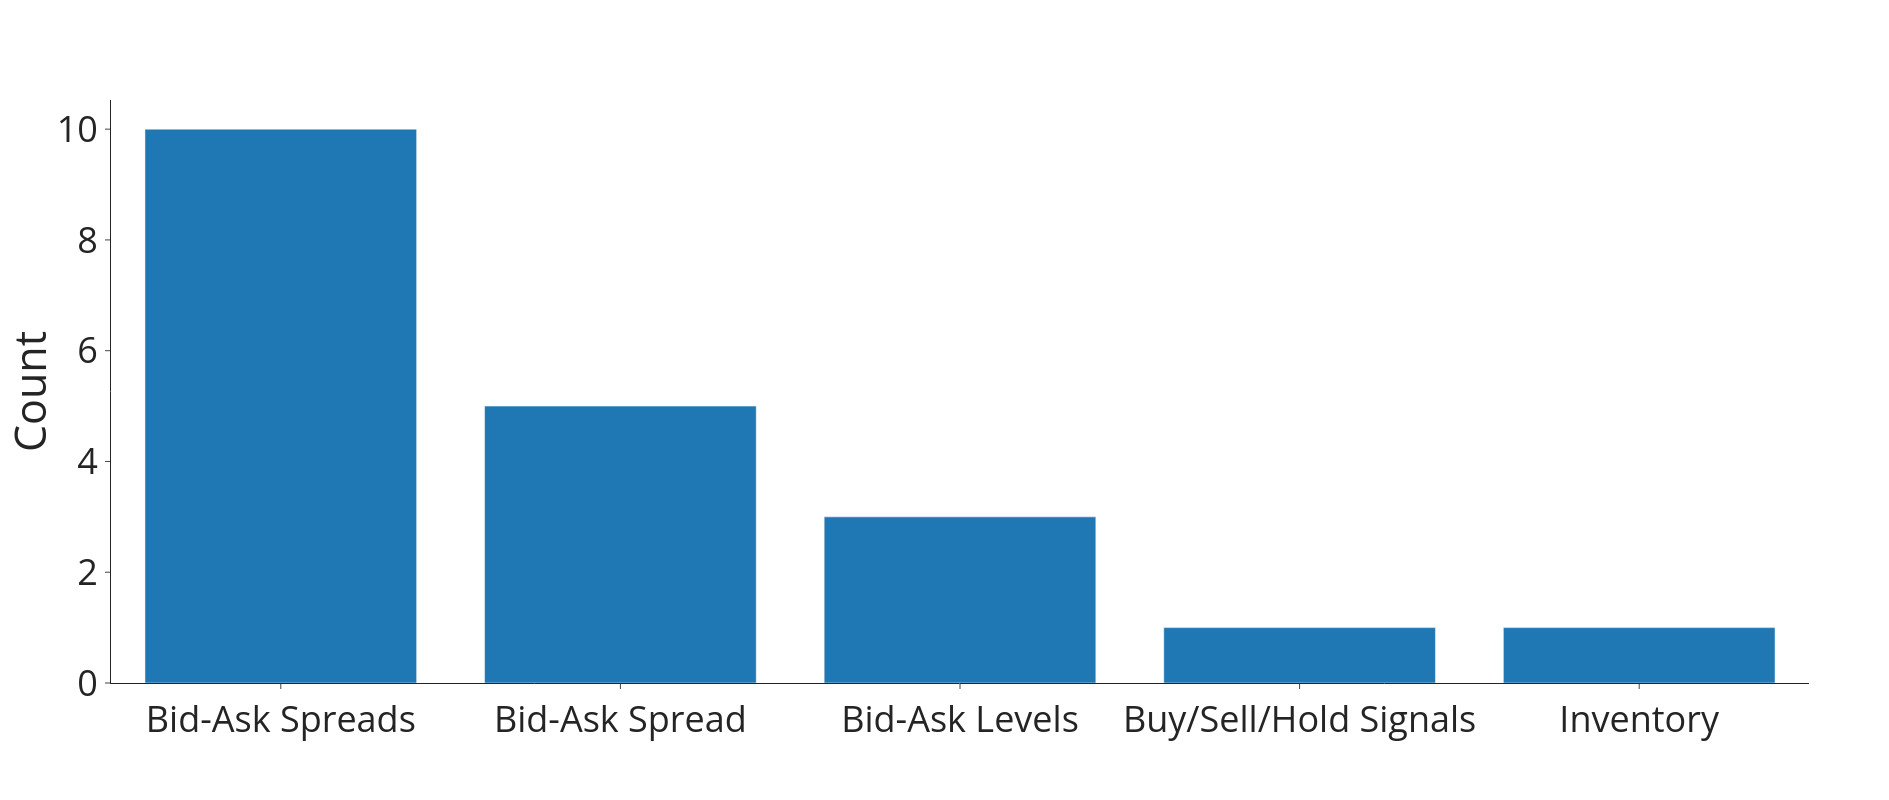
\includegraphics[width=\textwidth]{images/action_space}
            \caption{State Space 2}
            \label{fig:figure2}
        \end{subfigure}
    }
    \centering
    % graph: images/state_space.png
    \makebox[\textwidth][c]{%
        \begin{subfigure}{0.7\textwidth}
            \centering
            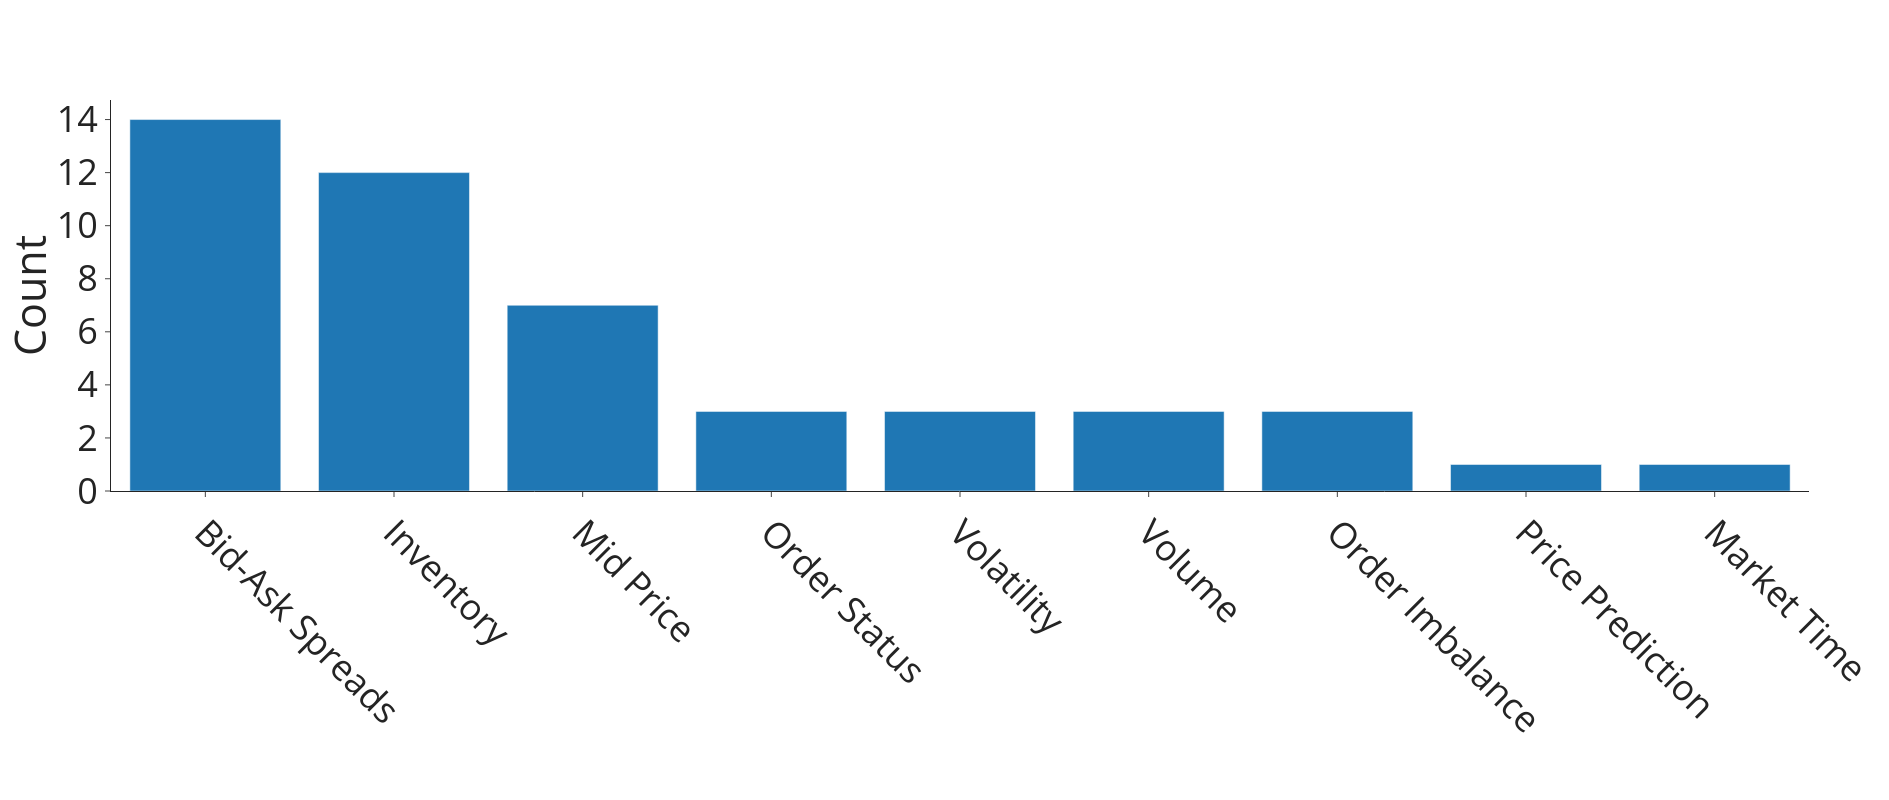
\includegraphics[width=\textwidth]{images/state_space}
            \caption{State Space 1}
            \label{fig:figure1}
        \end{subfigure}
    }
\end{figure}

Finally, almost all reward structures used some form of PnL and end-of-day liquidation or inventory penalties,
mostly due to the need to balance profitability and inventory risk \cite{sun2020marketmaking, gasperov2021marketmaking}.
However, the inclusion of additional explicit constraints or reward penalties, such as inventory and overnight risk penalties was rarely discussed or mentioned,
even though being essential to ensure practical applicability and risk management in live trading scenarios \cite{jerome2022modelbased, selser2021optimal}.

\subsection{Algorithms and Performance Metrics}
Recent trends in reinforcement learning research emphasize model-free approaches, particularly Deep Q-Learning and Actor-Critic methods,
which leverage neural networks to approximate value functions or policies to deal with the high-dimensional nature of limit order books \cite{patel2018optimizing, ganesh2019reinforcement}.
The literature showed that model-free approaches had strong adaptability capabilities towards changing market conditions while still maintaining acceptable training times.

\begin{figure}[H]
    \centering
    % graph: images/state_space.png
    \makebox[\textwidth][c]{%
        \begin{subfigure}{.5\textwidth}
            \centering
            \includegraphics[width=\textwidth]{images/reward_space}
            \caption{State Space 3}
            \label{fig:figure4}
        \end{subfigure}
        \hspace{0.02\textwidth} % Adjust spacing between figures
        \begin{subfigure}{0.5\textwidth}
            \centering
            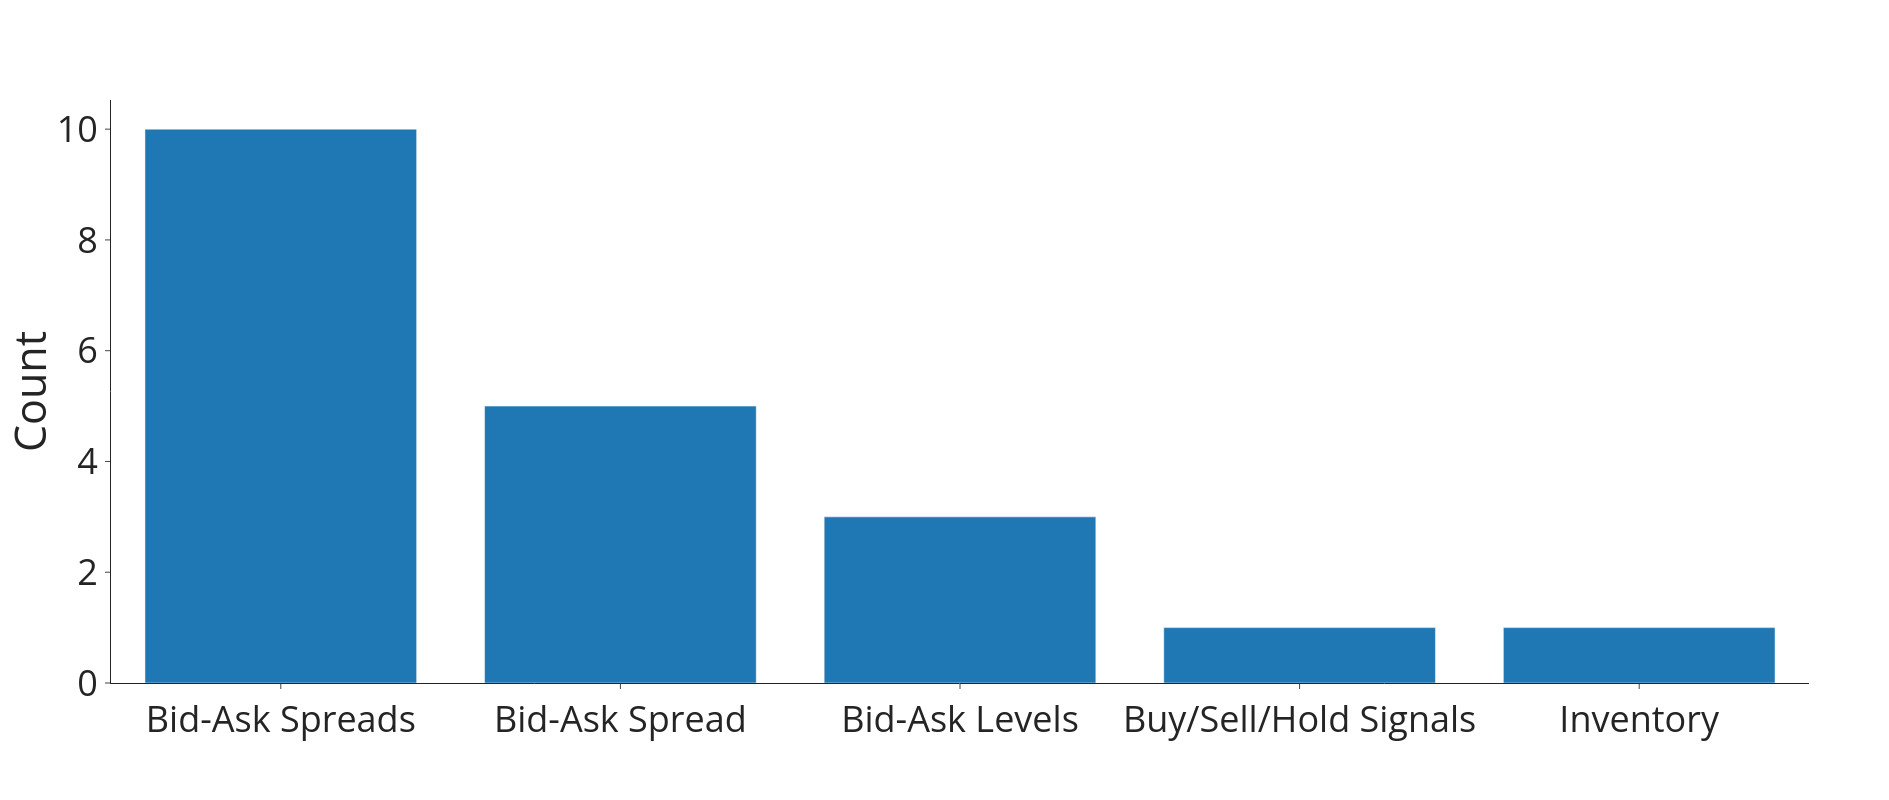
\includegraphics[width=\textwidth]{images/action_space}
            \caption{State Space 2}
            \label{fig:figure5}
        \end{subfigure}
    }
\end{figure}

The use of overnight position penalties was also mentioned in only 3 references, which leads to worse long-term sharpe ratios of the proposed strategies \cite{gasperov2021marketmaking}.

In summary, the bibliographical review underscores the relevance of reinforcement learning in optimizing market-making strategies,
particularly when combined with realistic state, action, and reward spaces.
The insights gained from this review inform the choice of the spaces used in this paper, as well as the design of our proposed restriction-based RL framework,
which seeks to enhance the stability and interpretability of market-making algorithms specifically addressing overnight risk and inventory constraints.
